\documentclass[a4paper,12pt]{article}
\usepackage[swedish]{babel}
\usepackage[utf8]{inputenc}
\usepackage{amsmath, amsthm, amssymb}
\usepackage{graphicx}
\usepackage{enumitem}
\usepackage[a4paper,includeheadfoot,margin=2.54cm]{geometry}
\usepackage{fancyhdr}
\pagestyle{fancy}
\fancyhead[R]{Zacharias Brohn - 9907174297}
\renewcommand{\headrulewidth}{0pt}
\setlength{\headheight}{14.5pt}
%
\begin{document}
%
\section*{Dugga 7 - Fråga 5}
Lös rekurrensekvationen
\begin{align}
    x_{n+2} - x_{n+1} - 2x_n = 3^n, \quad x_0 = 0, \quad x_1 = 1
\end{align}
%
\subsection*{Lösning}
För att lösa detta, börjar vi med att anta att högerledet är noll för att få den homogena ekvationen
\begin{align}
    x_{n+2} - x_{n+1} - 2x_n = 0.
\end{align}
%
\subsection*{Karakteristiska ekvationen}
Vi antar en lösning av formen $x_n = r^n$ och sätter in det i den homogena ekvationen
\begin{align}
    r^{n+2} - r^{n+1} - 2r^n = 0
\end{align}
Genom att dividera med $r^n$ (för $r \neq 0$) får vi
\begin{align}
    r^2 - r - 2 = 0
\end{align}
Vi löser kvadratisk ekvation
\begin{align}
    r = \frac{1 \pm \sqrt{1^2 - 4 \cdot 1 \cdot (-2)}}{2} = \frac{1 \pm \sqrt{9}}{2} = \frac{1 \pm 3}{2}
\end{align}
Detta ger rötterna
\begin{align}
    r_1 = 2, \quad r_2 = -1.
\end{align}
%
\subsection*{Den homogena lösningen}
Den allmänna lösningen till den homogena ekvationen blir
\begin{align}
    x_n^h = C_1 \cdot 2^n + C_2 \cdot (-1)^n,
\end{align}
där $C_1$ och $C_2$ är konstanter.
%
\subsection*{Partikulärlösning}
Eftersom högerledet är $3^n$, gissar vi en partikulärlösning av formen:
\begin{align}
    x_n^p = A \cdot 3^n
\end{align}
Vi sätter in $x_n^p$ i originalekvationen
\begin{align}
    A \cdot 3^{n+2} - A \cdot 3^{n+1} - 2A \cdot 3^n = 3^n
\end{align}
Förenkla exponenterna
\begin{align}
    9A \cdot 3^n - 3A \cdot 3^n - 2A \cdot 3^n = 3^n
\end{align}
Samla termer
\begin{align}
    (9A - 3A - 2A) \cdot 3^n = 3^n
\end{align}
Detta ger
\begin{align}
    4A \cdot 3^n = 3^n
\end{align}
Lös för $A$ genom att dividera båda led med $3^n$
\begin{align}
    4A = 1 \implies A = \frac{1}{4}
\end{align}
Den totala lösningen är summan av den homogena och partikulära lösningen
\begin{align}
    x_n = x_n^h + x_n^p = C_1 \cdot 2^n + C_2 \cdot (-1)^n + \frac{1}{4} \cdot 3^n.
\end{align}
%
\subsection*{Konstanterna}
För $n = 0$
\begin{align}
    x_0 = C_1 \cdot 2^0 + C_2 \cdot (-1)^0 + \frac{1}{4} \cdot 3^0 = C_1 + C_2 + \frac{1}{4} = 0 \label{eq:villkor1}
\end{align}
För $n = 1$
\begin{align}
    x_1 = C_1 \cdot 2^1 + C_2 \cdot (-1)^1 + \frac{1}{4} \cdot 3^1 = 2C_1 - C_2 + \frac{3}{4} = 1 \label{eq:villkor2}
\end{align}
%
Från ekv. \ref{eq:villkor1}
\begin{align}
    C_1 + C_2 = -\frac{1}{4} \label{eq:ekvC1}
\end{align}
Från ekv. \ref{eq:villkor2}
\begin{align}
    2C_1 - C_2 = \frac{1}{4} \label{eq:ekvC2}
\end{align}
Adderar ekvationerna:
\begin{align}
    (C_1 + C_2) + (2C_1 - C_2) = -\frac{1}{4} + \frac{1}{4}
\end{align}
Detta ger:
\begin{align}
    3C_1 = 0 \implies C_1 = 0
\end{align}
Sätt in $C_1 = 0$ i ekv. \ref{eq:ekvC1}
\begin{align}
    0 + C_2 = -\frac{1}{4} \implies C_2 = -\frac{1}{4}.
\end{align}
%
\subsection*{Lösningen}
Sätt in värdena för $C_1$ och $C_2$
\begin{align}
    x_n = 0 \cdot 2^n - \frac{1}{4} \cdot (-1)^n + \frac{1}{4} \cdot 3^n
\end{align}
Och genom att förenkla detta löser vi rekurrensekvationen
\begin{align}
    x_n = -\frac{1}{4} \cdot (-1)^n + \frac{1}{4} \cdot 3^n.
\end{align}
%
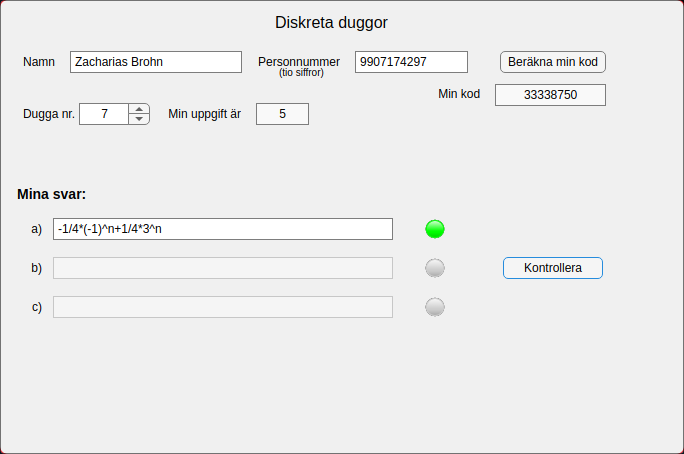
\includegraphics[width=\textwidth]{x3onjw9.png}
%
\end{document}